\chapter{Data preparation}
\label{ch:data_preparation}


Having cleaned the dataset and analysed the distribution of skin tone groups and malignant samples in it, we were ready to prepare the dataset for training. When splitting the data into training and validation subsets, we had to be careful not to introduce any further imbalance into the data, and make sure all skin groups were well represented across splits. As data exploration from chapter \ref{ch:data_understanding} revealed that the brown group was underpopulated, we decided to merge that group with the tan one. Furthermore, the ISIC2020 dataset is known to have duplicate images, so a total of 425 of them were removed before training. The resulting number of samples in each subset of our data for our chosen split strategy is shown in Table \ref{tab:data-split}. The following sections cover different augmentation and sampling techniques used in our experiments to synthetically balance the dataset and increase fairness.

\begin{table}[]
\centering
\caption{Image counts in the used train and validation splits for different skin tone groups.}
\label{tab:data-split}

\begin{tabular}{@{}lllrrc@{}}
\toprule
\multicolumn{2}{l}{\textbf{Skin tone group}}       & \textbf{Target} & \multicolumn{1}{l}{\textbf{Training}} & \multicolumn{1}{l}{\textbf{Validation}} & \multicolumn{1}{l}{\textbf{Ratio}} \\ \midrule
\multirow{2}{*}{0} & \multirow{2}{*}{Very light}   & benign          & 1072                                  & 268                                     & 4:1                                \\
                   &                               & malignant       & 16                                    & 17                                      & 1:1                                \\
\multirow{2}{*}{1} & \multirow{2}{*}{Light}        & benign          & 17515                                 & 4379                                    & 4:1                                \\
                   &                               & malignant       & 231                                   & 58                                      & 4:1                                \\
\multirow{2}{*}{2} & \multirow{2}{*}{Intermediate} & benign          & 62774                                 & 1569                                    & 4:1                                \\
                   &                               & malignant       & 181                                   & 46                                      & 4:1                                \\
\multirow{2}{*}{3} & \multirow{2}{*}{Tan + Brown}  & benign          & 834                                   & 209                                     & 4:1                                \\
                   &                               & malignant       & 16                                    & 16                                      & 1:1                                \\ \bottomrule
\end{tabular}
\end{table}

\section{Preprocessing}

We built our custom dataset, which we named LocalISICDataset. Images were loaded using a standard classification convention, where the data is split into train and valid directories, each containing class-named subfolders with the respective images.

Images were resized to 224×224 by default. We explored higher resolutions only for models that showed strong baseline performance, aiming to boost evaluation metrics. An exception was the DINOv2 model, which was pretrained on 518×518 images, so we used that crop size to extract feature representations for it.

Our dataset supported heavy augmentation, and we had several configurable options when creating it.
One could:

\begin{itemize}
    \item define malignant-class-only transformations, aiming to artificially oversample the minority class,
    \item define transformations to apply to all images (by default, this only included resizing to the target size),
    \item enable lesion segmentation: we generated segmentation masks of lesions where only the lesion region was retained and the rest of the image was blacked out,
    \item choose to convert images to the CIELAB color space: this introduced additional dataloading time, as we chose to perform the conversion on-the-fly, without saving pre-converted versions,
    \item apply skin darkening transformations in the CIELAB color space, as proposed in \cite{assessing_bias_in_classifiers}.
    \item apply normalization, which differed when using images in original RGB colorspace or images transformed in CIELAB colorspace.
\end{itemize}

\subsection{Segmentation masks}
As described in \ref{ch:data_understanding}, the segmentation procedure is image processing-based and includes contrast increase with CLAHE, hair removal using DullRazor and morphologically expanded Otsu thresholding to remove skin pigmentations

It is worth noting that our threshold segmentation method is sometimes prone to incorrectly identifying image edges as part of the lesion.

\vspace{1em}
\begin{figure}[htbp]
\centering
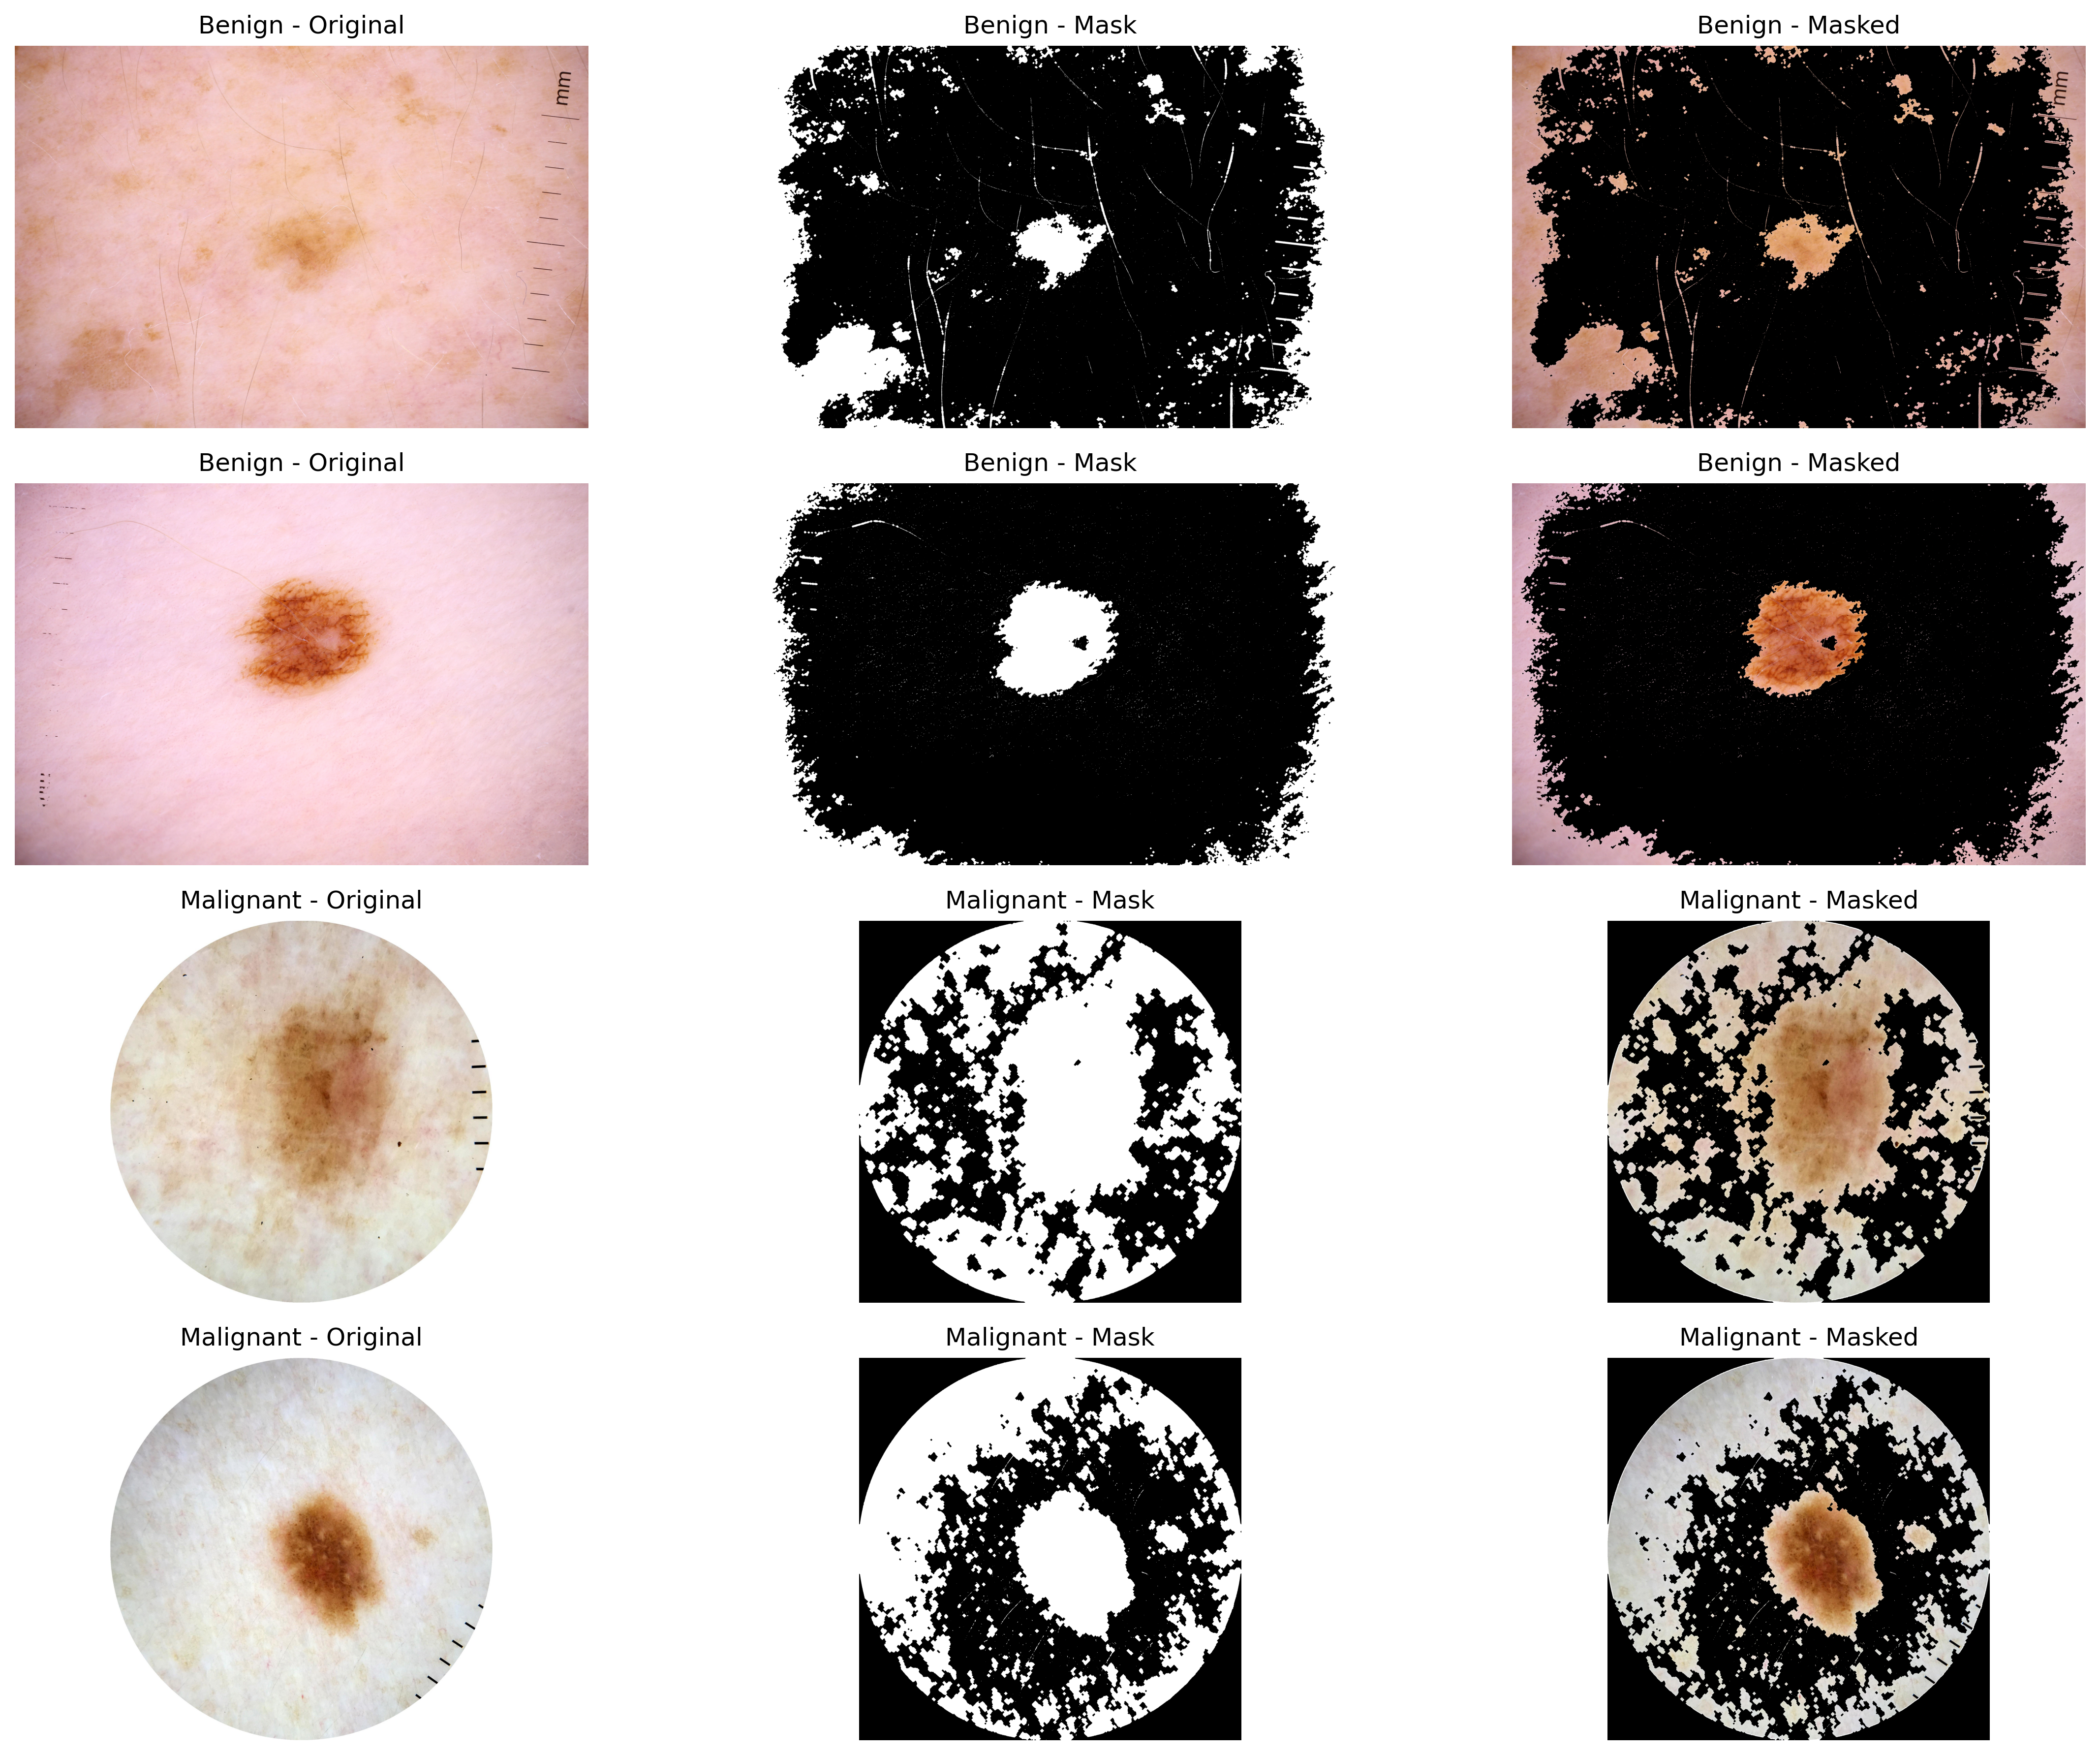
\includegraphics[width=\linewidth]{figures/dermoscopy_visualization.png}
\caption{Examples of benign and malignant images, their corresponding segmentation masks, and how segmentation-aided model inputs look after masking.}
\label{fig:segmentation-aided-inputs}
\end{figure}

\subsection{Segmentation masks in CIELAB}

To showcase an example of an image in the CIELAB color space and to demonstrate how masking appears in that space, we provide a visualization of a masked image:

\vspace{1em}
\begin{figure}[htbp]
\centering
\includegraphics[width=\linewidth]{figures/cielab_masked_image.jpeg}
\caption{Example of an image in CIELAB color space (visualized as RGB) after applying lesion segmentation.}
\label{fig:segmentation-cieelab}
\end{figure}


\subsection{Skin-former}

We refer to the technique of darkening images in the CIELAB color space as \textit{Skin-former}, an augmentation method aimed at reducing per-skin-type bias that a classification model might exhibit, especially since the distribution of skin color types is heavily imbalanced \cite{skin_color_debiasing}.

Such an uneven distribution presents a significant challenge, as our objective is to build a skin-type-agnostic classifier, mitigating any bias the model may have toward majority skin types. ISIC dataset mainly comprises of lighter skin color images.

To implement this, images are first converted from the RGB color space to the CIELAB color space. The \( L \) (lightness) and \( b \) (yellow-blue hue) components are then modified to simulate different Fitzpatrick Skin Types (FSTs). The transformation is based on a randomly selected target ITA value within the range of the desired FST. The new \( L \) and \( b \) components are calculated using Equations~\ref{eq:ita_diff}, \ref{eq:b_adjustment}, and \ref{eq:l_adjustment}.

\begin{myequation}[H]
\caption{ITA difference between original and target skin tone}
\label{eq:ita_diff}
\[
\Delta \text{ITA} = \text{ITA}_{\text{original}} - \text{ITA}_{\text{target}}
\]
\end{myequation}

\begin{myequation}[H]
\caption{Adjustment of the \textit{b} component in LAB space}
\label{eq:b_adjustment}
\[
b = b + (\Delta \text{ITA} \cdot 0.5)
\]
\end{myequation}

\begin{myequation}[H]
\caption{Adjustment of the \textit{L} component in LAB space}
\label{eq:l_adjustment}
\[
L = L - (\Delta \text{ITA} \cdot 0.12)
\]
\end{myequation}

Example of a side-by-side comparison of images before and after this augmentation can be seen in \ref{ap:skin_former}, here we present an example of this transformation.

\begin{figure}[ht]
    \centering
    \begin{subfigure}[b]{0.45\textwidth}
        \includegraphics[width=\linewidth]{figures/skin_former/ISIC_0081956.jpg}
        \caption{Original image}
        \label{fig:original_image}
    \end{subfigure}
    \hfill
    \begin{subfigure}[b]{0.45\textwidth}
        \includegraphics[width=\linewidth]{figures/skin_former/ISIC_0081956.jpg_shifted.png}
        \caption{Image after skin-former transformation. ITA was reduced by 46.28°, changing group to Brown.}
        \label{fig:augmented_image}
    \end{subfigure}
    \caption{Side-by-side comparison of image before and after skin-former augmentation.}
    \label{fig:sidebyside_skinformer}
\end{figure}

\section{Data samplers}

There are many different approaches to balancing datasets, such as undersampling the majority class, oversampling the minority class, using the \textit{Synthetic Minority Oversampling Technique (SMOTE)}, applying data augmentation strategies, or generating new samples with GANs (e.g., \textit{DermaGAN}).

In our work, we decided to utilize three types of data samplers:
\begin{itemize}
    \item Balanced batch sampler
    \item Imbalanced dataset sampler
    \item Undersampler
\end{itemize}

It is important to highlight the key distinction between the oversampler and the balanced batch sampler. While both can be used to generate a balanced benign–malignant dataset, the balanced batch sampler enforces equal class representation within each individual batch. In contrast, the oversampler does not guarantee balanced batches, meaning that a balance could, for instance, be achieved through a batch of only positives followed by a batch of only negatives.

\subsection{Balanced batch sampler vs undersampler}

Balanced batch sampler creates random duplicate records of malignant class samples. Given that we already apply augmentation techniques to mitigate the 49-to-1 class imbalance in favor of the benign class, it is evident that this approach could lead to overfitting.
In contrast, the undersampler suffers from information loss issues, primarily because it is not known a priori which benign images are hard to classify. Randomly dropping samples from the dataset can cause the model to perform worse, especially since a large portion of the dataset must be discarded to bring the number of benign samples closer to the number of malignant ones.

\vspace{1em}
\begin{figure}[htbp]
\centering
\includegraphics[width=\linewidth]{figures/over_vs_under_sampler.png}
\caption{Over- vs undersampler visualization.}
\label{fig:over_under_sampler}
\end{figure}

\subsection{Imbalanced dataset sampler}

To tackle the severe class imbalance present in the ISIC 2020 dataset, we experimented with a smarter oversampling strategy by integrating the \texttt{ImbalancedDatasetSampler}\footnote{\url{https://pypi.org/project/torchsampler/}} from the \texttt{torchsampler} library. This PyTorch sampler rebalances class distributions dynamically during training, without modifying or duplicating the dataset. Additionally, it automatically estimates sampling weights based on class frequencies. It avoids the need to create a new balanced dataset upfront, and when used with data augmentation, it can help mitigate overfitting by increasing sample variety.


\vspace{1em}
\begin{figure}[htbp]
\centering
\includegraphics[width=0.5\linewidth]{figures/imbalanced_dataset_sampler.png}
\caption{Imbalanced dataset sampler visualization.}
\label{fig:imbalanced_dataset_sampler}
\end{figure}
